% !TEX root =  ../main_manuscript.tex 
\subsection{Statistical Model}
To create personalized biopsy schedules based on patient-specific risk of reclassification, we required a risk prediction model. Available data was patient age at inclusion in AS, PSA measurements over follow-up, the timing of repeat biopsies and corresponding Gleason grades, and observed time of reclassification. Analysis of this data required modeling the correlation between the PSA measurements of the same patient, the correlation between the Gleason grade and the PSA profile, and to account for PSA measurements missing after a patient experienced reclassification. To this end, a commonly used model is the joint model for time-to-event and longitudinal data \citep{tomer2019,coley2017prediction,rizopoulos2012joint}.

Our joint model consisted of two sub-models. First, a linear mixed model \citep{laird1982random} for longitudinally measured PSA (log-transformed). Second, a relative-risk model (similar to Cox model) for obtaining the risk of reclassification. In the model for PSA, we fitted a curve to PSA measurements (Panel~A, Figure~\ref{fig:jmExplanationPlot_113}). From each patient's fitted PSA profile we extracted the instantaneous PSA velocity. This velocity varies over time (Panel~B, Figure~\ref{fig:jmExplanationPlot_113}). Consequently, it is more precise than the currently used definition of PSA velocity \citep{vickers2009psavelocity}. We connected the two sub-models by using the fitted PSA and instantaneous velocity as predictors in the sub-model for risk of reclassification (Panel~C, Figure~\ref{fig:jmExplanationPlot_113}). Patient age was included in both sub-models. The parameters of the two sub-models were estimated jointly (Appendix~A) using the R package \textbf{JMbayes} \citep{rizopoulosJMbayes}. 

\begin{figure}
\centerline{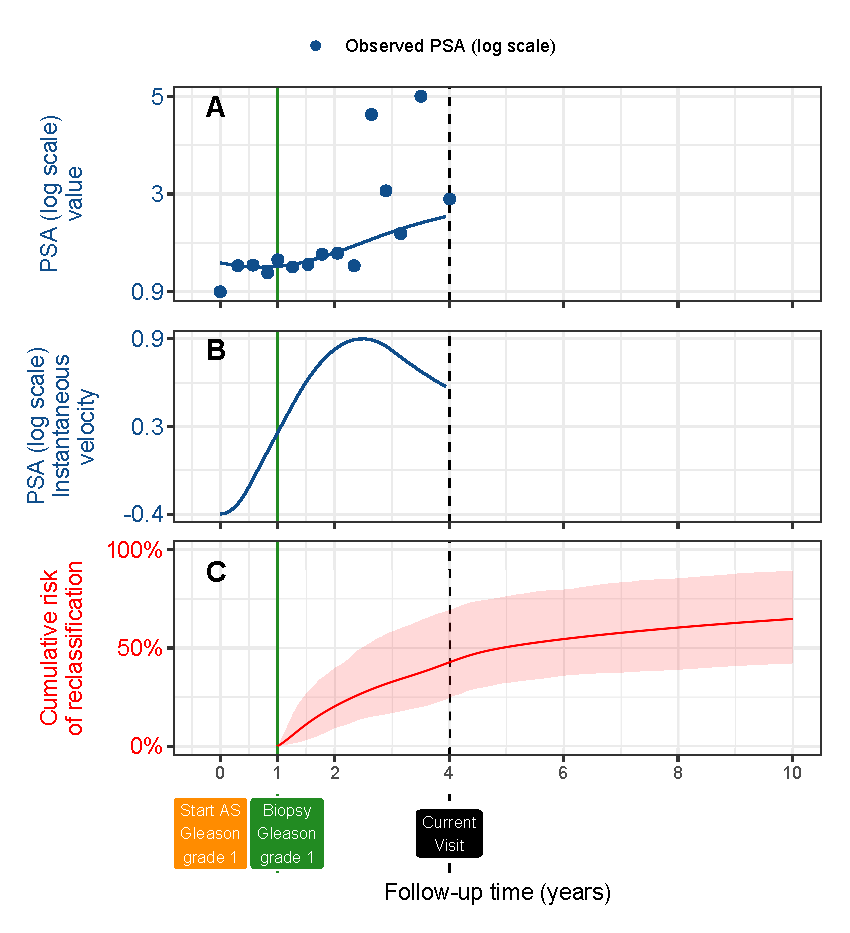
\includegraphics[width=\columnwidth]{images/jmExplanationPlot_113.eps}}
\caption{\textbf{Illustration of the joint model on a real PRIAS dataset patient}. \textbf{Panel~A:} Observed (blue dots) and fitted PSA (solid blue line) measurements, log-transformed. \textbf{Panel~B:} Estimated instantaneous velocity of PSA (log-transformed). \textbf{Panel~C}: Predicted cumulative-risk of reclassification (95\% credible interval shaded). Reclassification is defined as increase in Gleason grade \citep{epsteinGG2014} from grade~1 to 2 or higher. This risk of reclassification is available starting from the time of the latest negative biopsy (vertical green line at year 1 of follow-up). Joint model estimated it by combining the fitted PSA value and velocity (both on log scale of PSA) and time of latest negative biopsy. Black dashed line at year 4 denotes time of current visit.}
\label{fig:jmExplanationPlot_113}
\end{figure}

\subsection{Predicting Risk of Reclassification}
The key component in personalized schedules is the cumulative-risk of reclassification. Given, a patient's PSA measurements and previous biopsy results, our joint model predicts the cumulative-risk of reclassification at his current as well as future visit times (e.g., Panel~C, Figure~\ref{fig:jmExplanationPlot_113}). The cumulative-risk profile is also updated as more patient data becomes available over follow-up (Appendix B).

We validated our model internally as well as externally. Internal validation was done using PRIAS dataset. External validation was done in largest five AS cohorts from the GAP3 database \citep{gap3_2018}, namely University of Toronto AS (Toronto-AS), Johns Hopkins AS (JH-AS), Memorial Sloan Kettering Cancer Center AS (MSKCC-AS), King's College London AS (KCL-AS), and Michigan Urological Surgery Improvement Collaborative AS (MUSIC-AS). We assessed our model's discrimination via the area under the receiver operating characteristic curve or AUC \cite{rizopoulos2017dynamic}. For calibration we utilized calibration plots for visual assessment, and root mean squared prediction error \cite{rizopoulos2017dynamic} for quantitative assessment. We also recalibrated our model's baseline hazard of reclassification for each of the five external cohorts (Appendix B).

\subsection{Personalized Biopsy Schedules}
We created personalized schedules of biopsies upon a patient's visit for testing PSA (every 6 months in PRIAS). Specifically, if a patient's cumulative-risk of reclassification at his current PSA visit was more than a certain threshold (e.g., 10\%) we scheduled an immediate biopsy. Our model predicted his cumulative-risk of reclassification at his future PSA follow-up visits as well. Thus, by applying the same risk threshold rule at each future follow-up visit, we scheduled future biopsies (Appendix C). We kept a minimum gap of one year between consecutive biopsies (PRIAS recommendation). Example personalized schedules based on different risk thresholds are shown in Figure~\ref{fig:demo_pat1}.

The choice of the risk threshold in the personalized schedule dictates the \textit{consequences} of following that schedule. \textit{Consequences} are the timing and the total number of biopsies, and the expected delay in detecting reclassification. Larger risk thresholds will schedule infrequent personalized biopsies. However, the consequent delay in detecting reclassification may also be longer. Our model also estimated these \textit{consequences} in a personalized manner given any schedule of biopsies. Thus patients can compare fixed schedules with various risk threshold based personalized schedules before making a choice.

\subsection{Web-Application}
We implemented our methodology in a web-application \url{https://emcbiostatistics.shinyapps.io/prias_biopsy_recommender/}. It utilizes our joint model fitted to the PRIAS dataset. Currently, the web-application supports PRIAS and the five external cohorts in which we validated our model. Patient data can be entered manually or can be uploaded in Microsoft Excel format. Predictions for risk of reclassification are shown for the first ten years of follow-up only (current study period of PRIAS). The web-application shows the \textit{consequences} of following these schedules: personalized schedules based on 5\%, 10\%, and 15\% risk threshold; annual biopsies; biennial biopsies; and PRIAS schedule.

\begin{figure}[!htb]
\centerline{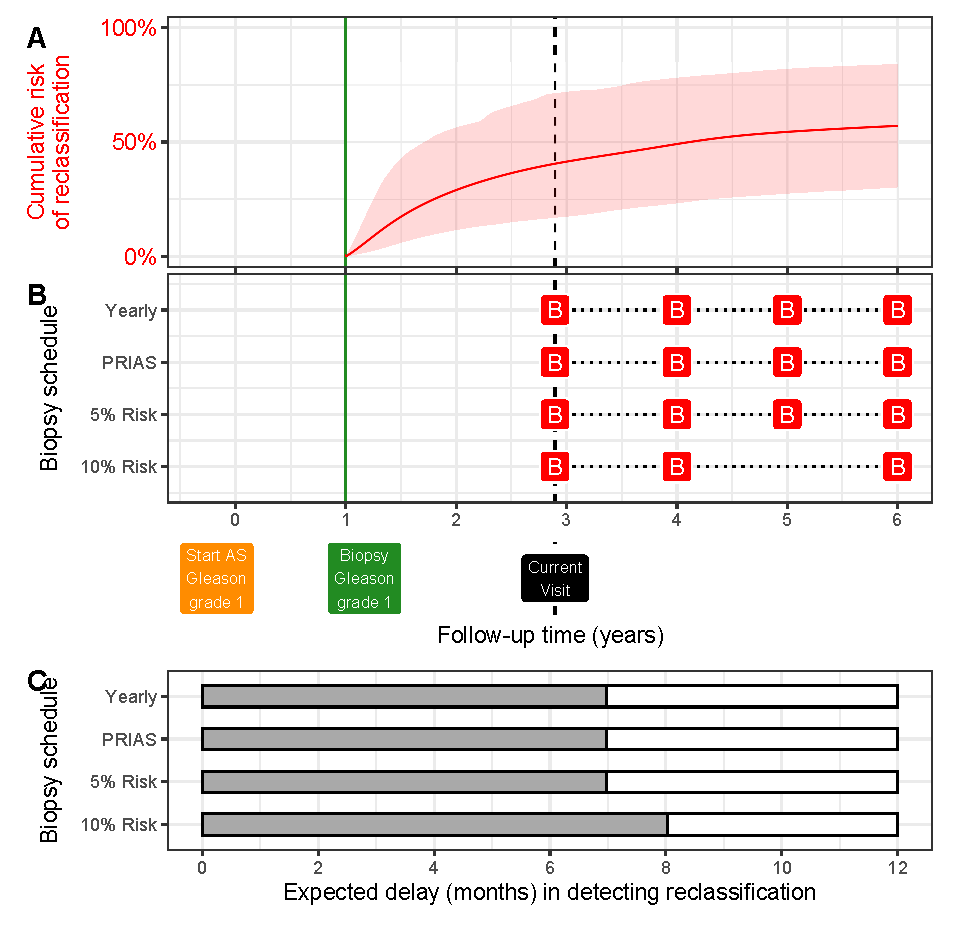
\includegraphics[width=\columnwidth]{images/demo_pat1.eps}}
\caption{\textbf{Illustration of personalized and fixed schedules of biopsies}. The PSA profile of this patient is shown in Figure~\ref{fig:jmExplanationPlot_113}. \textbf{Panel~A:} Predicted cumulative-risk of reclassification (95\% credible interval shaded). \textbf{Panel~B:} Personalized and fixed schedules of biopsies, with a red `B' indicating a scheduled biopsy. \textbf{Panel~C:}\ Expected delay in detecting reclassification for different schedules. Green vertical line at year 1 denotes time of latest negative biopsy. Black dashed line at year 4 denotes time of current visit.}
\label{fig:demo_pat1}
\end{figure}